\documentclass[12pt,addpoints,answers]{exam}
\usepackage[utf8]{inputenc}

\unframedsolutions
\renewcommand{\solutiontitle}{\noindent\textbf{Solution:}\par\noindent}
\SolutionEmphasis{\color{blue}}
\noprintanswers

\usepackage{booktabs}
\usepackage{tabularx}
\usepackage{xfrac}

\usepackage{siunitx}
\sisetup{parse-numbers=false}

\usepackage{listings}
\lstset{basicstyle=\scriptsize\ttfamily}

\usepackage{tikz}
\usetikzlibrary{arrows}
\usetikzlibrary{decorations.pathreplacing}
\usetikzlibrary{chains}
\usetikzlibrary{positioning}
%\tikzset{>=stealth',every on chain/.append style={join}, every join/.style={-,blue,thick,dashed}}



\title{Computer Networks Homework 1}
\author{Fall 2019}
\date{Due: 3 February 2020}

\begin{document}
\maketitle

\begin{questions}
\question[12] Imagine that there are two paths a packet could take to travel from Host $J$ to Host $K$, as illustrated here:
\begin{center}
\begin{tikzpicture}[
	node distance=1.00in
]
\node[label=below:{\scriptsize{Host A}}]                                          (hostA)     {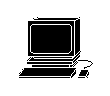
\includegraphics[scale=0.5]{fig/cisco/workstation}};
\node[label=above:{\scriptsize{Switch}}, right of=hostA]                          (switchA.1) {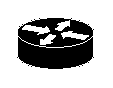
\includegraphics[scale=0.5]{fig/cisco/router}};
\node[label=above:{\scriptsize{Switch}}, right of=switchA.1, node distance=1.5in] (switchA.2) {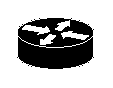
\includegraphics[scale=0.5]{fig/cisco/router}};
\node[label=above:{\scriptsize{Switch}}, right of=switchA.2, node distance=1.5in] (switchA.3) {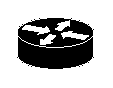
\includegraphics[scale=0.5]{fig/cisco/router}};
\node[label=below:{\scriptsize{Switch}}, below of=switchA.1, node distance=0.5in] (switchB.1) {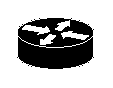
\includegraphics[scale=0.5]{fig/cisco/router}};
\node[label=below:{\scriptsize{Switch}}, right of=switchB.1]                      (switchB.2) {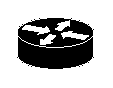
\includegraphics[scale=0.5]{fig/cisco/router}};
\node[label=below:{\scriptsize{Switch}}, right of=switchB.2]                      (switchB.3) {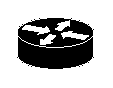
\includegraphics[scale=0.5]{fig/cisco/router}};
\node[label=below:{\scriptsize{Switch}}, right of=switchB.3]                      (switchB.4) {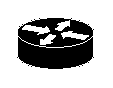
\includegraphics[scale=0.5]{fig/cisco/router}};
\node[label=below:{\scriptsize{Host B}}, right of=switchA.3]                      (hostB)     {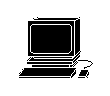
\includegraphics[scale=0.5]{fig/cisco/workstation}};
\begin{scope}[start chain,>=stealth',every on chain/.append style={join}, every join/.style={-,blue,thick,dashed}]
	\chainin (hostA);
	\chainin (switchA.1);
	\chainin (switchA.2);
	\chainin (switchA.3);
	\chainin (hostB);
\end{scope}
\begin{scope}[start chain,>=stealth',every on chain/.append style={join}, every join/.style={-,red,thick}]
	\chainin (switchA.1);
	\chainin (switchB.1);
	\chainin (switchB.2);
	\chainin (switchB.3);
	\chainin (switchB.4);
	\chainin (switchA.3);
\end{scope}
\end{tikzpicture}
\end{center}
Each link drawn with a dashed blue line has a bandwidth of \SI{250000}{bps}; each link drawn with a solid red line has a bandwidth of \SI{400000}{bps}. Packets are always \SI{1000}{bytes}. You may assume that process, queue, and propegation delays are negligable.

What is the delay in each path? Which path should the packet take to get to Host $K$ the fastest?
\begin{solution}
\end{solution}

\question[8] Consider again the network in Question 1. Each link drawn with a dashed blue line still has a bandwidth of \SI{250000}{bps}. What is the minimum bandwidth for solid red links such that the bottom path is faster than the top path?
\begin{solution}
\end{solution}

\question[12] A mountain bike rider is competing in the Tour Divide, a \SI{4418}{\kilo\meter} race from Banff, Alberta to Antelope Wells, New Mexico. She is carrying a GPS tracker, as do all racers. The tracker sends a signal to a satellite, which relays it back down to a server in New Orleans, LA. A friend of this rider wants to know her current position. What is the delay from when the signal leaves the tracker to when the friends computer in Seattle, Washington?

Assume the following:
\begin{enumerate}
\item the connection from the tracker to the satellite (and the satellite back to the server) is wireless and the signal travels at the speed of light,
\item the satellite is orbiting in medium-Earth orbit at approximately \SI{20000}{\kilo\meter},
\item the friend is using a copper connection to retieve the information,
\item it is approximately \SI{4228}{\kilo\meter} from New Oreleans to Seattle, and finally,
\item the transmission delay of the packet of the packet is negligible because it is so small.
\end{enumerate}
\begin{solution}
\end{solution}

\question[12] A security camera captures images that are each \SI{100000}{bytes} in size. It takes one image every \SI{.25}{\second}. If there is a \SI{500}{\meter} point-to-point (cable, $\SI{2.3 \cdot 10^8}{bps}$ propegation rate) connection to the monitor where the security guard inspects these images, what is the minimum acceptable bandwidth (bandwidth required to transmit one image before the next is taken) between the camera and monitor?
\begin{solution}
\end{solution}

\question[8] A standard Ethernet frame (or packet) is \SI{1500}{bytes}. The most common version of Ethernet found on consumer devices is Gigabit Ethernet, which operates with a bandwidth of \SI{1}{Gbps}. If two hosts are placed \SI{2500}{\meter} away from each other, how many frames should be sent out to ``peek the pipe full'' for the full Round Trip Time?
\begin{solution}
\end{solution}

\question Let's think a little about security in my analogy of sending a multi-part present to Samantha. Suggest mechanisms to accomplish each of the following tasks below. Remember that we are protecting physical packages, not packets!
\begin{parts}
\part[4] I don't want the post office to know who the source of the presents is, but I want Samantha and her mom to know.
\part[4] I don't want anybody except Samantha to know who the source of the presents is.
\part[4] Even if the postal worker opens up the packages, I don't wnat him to know that the three packages are related.
\end{parts}
\begin{solution}
\end{solution}

\question[8] A standard Ethernet frame has a payload of \SI{1500}{octets}. I have designed an application-layer protocol with a fixed 16 octets of header data. Use any reliable resource to find the standare header sizes for TCP and IP. What is the maximum actual data that can fit into the payload of that Ethernet frame after all the headers? What is the percentage overhead?
\begin{solution}
\end{solution}

\question[8] Shown below is a simple HTTP GET request with some cookie values. What is the ultimate address that is requested by the client? (You may have to make some assumptions about how the server interprets the cookies. State these assumptions and make them logical!)\\
\begin{minipage}{\textwidth}
\begin{lstlisting}[language={},escapechar=§,basicstyle=\ttfamily,breaklines=true]
GET /pages/home.html HTTP/1.1
Host: www.mtu.edu
Connection: close
User-Agent: Mozilla/5.0 (Macintosh; Intel Mac OS X 10_14_6) AppleWebKit/537.36 (KHTML, like Gecko) Chrome/76.0.3809.132 Safari/527.36
Cookie: user=newton
Cookie: dept=ECE
Cookie: userprefixchar=%7E
\end{lstlisting}
\end{minipage}
\begin{solution}
\end{solution}

\question[8] Show a full HTTP response message for a simple HTML document that just has the text, ``Hello, World!'' as its sole content. Send two cookies to the client: a random session key called PersonID; and a cookie called Planet with the value ``Earth'' that expires on January 1, 2099 at 11:59 pm.
\begin{solution}
\end{solution}

\question[12] A somewhat smart browser makes an initial request for a webpage an closes the connection. After parsing the requested page, it will make several consecutive requests for the images without closing the connection. If the webpage below shows the HTML page requested by the original request, show the subsequent request and response messages. You do not need to make up data for the images, but get the Content Type correct!\\
\begin{minipage}{\textwidth}
\begin{lstlisting}[language={},escapechar=§,basicstyle=\ttfamily,breaklines=true]
<HTML>
  <HEAD>
    <TITLE>My Vacation Pictures</TITLE>
  </HEAD>
  <BODY>
    <H1>Pictures from my vacation to Japan!</H1>
    <IMG src=GoldenPavillion.png>
    <br>
    <IMG src=food.jpg>
    <br>
    <IMG src=Geisha.png>
    <br>
  <BODY>
</HTML>
\end{lstlisting}
\end{minipage}

\begin{solution}
\end{solution}

\end{questions}
\end{document}
